\begin{frame}
  \frametitle{¿Qué es un Sistema Operativo?}
  \begin{itemize}
	  \item Es parte esencial de cualquier sistema de cómputo
	  \item Es un programa que actúa, en principio, como intermediario entre el usuario y el hardware
	  \item Su propósito: crear un entorno cómodo y eficiente para la ejecución de programas
	  \item Su obligación: garantizar el correcto funcionamiento del sistema
	  \item Sus funciones principales
		  \begin{itemize}
			  \item Administrar la memorio
			  \item Administrar la CPU
			  \item Administrar los dispositivos
		  \end{itemize}
  \end{itemize}
\end{frame}

\begin{frame}{¿Qué es un Sistema Operativo? (cont.)}
  \begin{itemize}
  \item Según Wikipedia:
  
   \textit{``...Es un conjunto de programas de computación destinados a realizar muchas tareas...''}
  \item Según un usuario stándar: ``Lo que aparece cuando prendo la PC''
  \item ...
  \end{itemize}
\end{frame}

\begin{frame}
	\frametitle{GNU/Linux}
	\begin{itemize}
		\item Es un Sistema Operativo tipo \textit{Unix} (Unix like), pero libre
		\item S.O. diseñado por miles de programadores
		\item S.O. gratuito y de libre distribución (se baja desde la Web, CD, etc.)
		\item Existen diversas distribuciones (customizaciones)
		\item \alert{Es código abierto}, lo que nos permite estudiarlo, personalizarlo, auditarlo, aprovecharnos de la documentación, etc...
	\end{itemize}
	\centerline{\alert{Podemos ver como está hecho!!!}}
\end{frame}

\begin{frame}
	\frametitle{¿GNU?}
	\begin{itemize}
		\item GNU = \textbf{G}NU \textbf{N}o es \textbf{U}nix
		\begin{figure}
			\centering
			
\includegraphics[scale=0.2]{images/gnu.png}
		\end{figure}
		\item Iniciado por \emph{Richard Stallman} en 1983 con el fin de crear un Unix libre (el sistema GNU)
		\item Para asegurar que el mismo fuera libre, se necesitó crear un marco regulatorio conocido como GPL (General Public License de GNU)
		\item En 1985, Stallman crea la FSF (Free Software Foundation), con el fin de financiar el proyecto GNU
		\item En 1990, GNU ya contaba con un editor de textos (Emacs), un compilador (GCC) y gran cantidad de bibliotecas que componen un Unix típico.
		\item Pero aún seguía faltando el componente principal $\rightarrow$ El Núcleo (\textit{Kernel})
	\end{itemize}
\end{frame}

\begin{frame}
	\frametitle{¿GNU? (cont.)}
	\begin{itemize}
		\item Si bien ya se venía trabajando en un núcleo conocido como \textit{TRIX}, es en 1988 que se decide abandonarlo debido a su complejidad (corría en hardware muy costoso)
		\item En este momento se decide adoptar como base el núcleo \textit{MACH} para crear \textit{GNU Hurd}, el cual tampoco prosperó
		\item \emph{Linus Torvalds} ya venía trabajando desde 1991 en un Kernel denominado \textit{Linux}, el cual se distribuiría bajo licencia GPL
		\item En el año 1992, Torvalds y Stallman deciden fusionar ambos proyectos, y es allí donde nace \textit{GNU/Linux}
		\item GNU/Linux pertenece al desarrollo del software libre	
	\end{itemize}
\end{frame}

\begin{frame}
	\frametitle{¿GNU? (cont.)}
	\begin{itemize}
		\item GNU se refiere a 4 libertades principales de los usuarios del software:
		\begin{itemize}
			\item Libertad de usar el programa con cualquier propósito
			\item Libertad de estudiar su funcionamiento
			\item Libertad para distribuir sus copias
			\item Libertad para mejorar los programas
		\end{itemize}
		\center{\textit{``Los programas son una forma de expresión de ideas. Son propiedad de la humanidad y deben ser compartidos con todo el mundo''}}
	\end{itemize}
\end{frame}

\begin{frame}
	\frametitle{¿Software libre?}
	\begin{figure}
		\centering
		\fbox{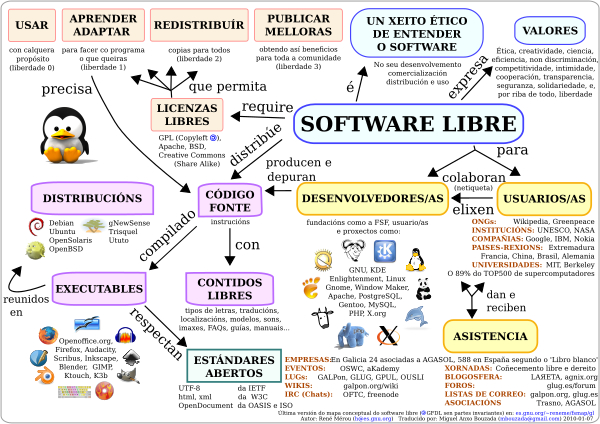
\includegraphics[scale=0.3]{images/freeSoft.jpg}}
	\end{figure}
\end{frame}

\begin{frame}
	\frametitle{¿Software libre?}
	\begin{itemize}
		\item Características del software libre:
		\begin{itemize}
			\item Una vez obtenido, puede ser usado, copiado, estudiado, modificado y redistribuido libremente
			\item Generalmente es de costo nulo $\leftarrow$ Es un gran error asociar el software libre con el software gratuito $\leftarrow$ Pensar en software gratis que se distribuye con restricciones
			\item Es común que se distribuya junto con su código fuente
			\item Corrección más rápida ante fallas
			\item Características que se refieren a la libertad de los usuarios para ejecutar, copiar, distribuir, estudiar, cambiar y mejorar el software
		\end{itemize}
	\end{itemize}
\end{frame}

\begin{frame}
	\frametitle{¿Software propietario?}
	\begin{itemize}
		\item Características del software propietario:
		\begin{itemize}
			\item Generalmente tiene un costo asociado
			\item No se lo puede distribuir libremente
			\item Generalmente no permite su modificación
			\item Normalmente no se distribuye junto con su código fuente
			\item La corrección de fallas esta a cargo del propietario
			\item Meno necesidad de técnicos especializados
		\end{itemize}
	\end{itemize}
\end{frame}

\begin{frame}
	\frametitle{GPL: Generic Public License}
	\begin{itemize}
		\item Licencia Pública General de GNU
		\item Creada en el año 1989 por la FSF
		\item Su objetivo principal es proteger la libre distribución, modificación y uso del software GNU
		\item Su propósito es declarar que todo software publicado bajo esta licencia es libre y esta protegido teniendo encuanta las 4 libertades principales ya vistas
		\item La versión actual de la licencia es la 3
	\end{itemize}
\end{frame}

\begin{frame}
	\frametitle{Características generales de GNU/Linux}
	\begin{itemize}
		\item Es multiusuario
		\item Es multitarea y multiprocesador
		\item Es altamente portable
		\item Posee diversos intérpretes de comandos, de los cuales algunos son programables
		\item Permite el manejo de usuarios y permisos
		\item Todo es un archivo (hasta los dispositivos y directorios)
		\item Cada directorio puede estar en una partición diferente (/temp, /home, etc.)		
		\item Es case sensitive
		\item Es código abierto
	\end{itemize}
\end{frame}

\begin{frame}
	\frametitle{Diseño}
	\begin{itemize}
		\item Fue desarrollado buscando la portabilidad de los fuentes
		\item Desarrollo en capas
		\begin{itemize}
			\item Separación de funciones
			\item Cada capa actúa como una caja negra hacia las otras
			\item Posibilita el desarrollo distribuido
		\end{itemize}
		\item Soporte para diversos File Systems
		\item Memoria virtual = RAM + \textit{SWAP}
		\item Desarrollo mayoritario en C y assembler
		\item Otros lenguajes: java, perl, python, etc.
	\end{itemize}
\end{frame}

\begin{frame}
	\frametitle{Estructura básica del S.O. - Núcleo}
	\begin{itemize}
		\item También conocido como \textit{Kernel}
		\item Ejecuta programas y gestiona dispositivos de hardware
		\item Es el encargao de que el software y el hardware puedan trabajar juntos
		\item Sus funciones más importantes son la administración de memoria, CPU y la E/S
		\item En si, y en un sentido estricto, es el sistema operativo
		\item Es un núcleo monolítico híbrido:
		\begin{itemize}
			\item Los drivers y código del Kernel se ejecutan en modo privilegiado
			\item Lo que lo hace híbrido es la capacidad de cargar y descargar funcionalidad a través de módulos
		\end{itemize}
		\item Está licenciado bajo la lecencia GPL v2
	\end{itemize}
\end{frame}

\begin{frame}
	\frametitle{Núcleo - Un poco de historia}
	\begin{itemize}
		\item En 1991 Linus Torvalds inicia la programacion de un Kernel \textit{Linux} basado en \textit{Minix} (clon de Unix desarrollado por \emph{Tenembaum} en 1987 con el fin de crear un S.O. de uso didáctico)
		\item El 5 de octubre de 1991, se anuncia la primera versión ``oficial'' de Linux (0.02)
		\item En 1992 se combina su desarrollo con GNU, formando GNU/Linux
		\item La versión 1.0 apareció el 14 de marzo de 1994
		\item Desarrollo continuado por miles de programadores al rededor del mundo
	\end{itemize}
\end{frame}

\begin{frame}
	\frametitle{Núcleo - Un poco de historia (cont.)}
	\begin{itemize}
		\item En mayo de 1996 se decide adoptar a \emph{Tux} como mascota oficial de Linux
		\begin{figure}
			\centering
			
\includegraphics[scale=0.1]{images/tux.png}
		\end{figure}
		\item En julio de 1996 se lanza la versión 2.0 y se define la nomenclatura de versionado. Se desarrolló hasta febrero de 2004 y terminó con la 2.0.40
		\item En enero de 1999 se lanza la versión 2.2, que proveé mejoras de portabilidad entre otras y se desarrolla hasta febrero de 2004 terminando en la versión 2.2.26
		\item En 2001 se lanza la versión 2.4 y se deja de desarrollar a fines del 2010 con la 2.4.37.11
		\begin{itemize}
			\item La versión 2.4 fue la que catapultó a GNU/Linux como un SO estable y robusto. Durante este período es que se comienza a utilizar Linux más asiduamente
		\end{itemize}
	\end{itemize}
\end{frame}

\begin{frame}
	\frametitle{Núcleo - Un poco de historia (cont.)}
	\begin{itemize}
		\item A fines del 2003 se lanza la versión 2.6		
		\item Esta versión ha tenido muchas mejoras para el SO dentro de las que se destacan soporte de hilos, mejoras en la planificación y soporte de nuevo hardware
		\item El 3 de agosto de 2011 se lanza la versión 2.6.39.4
		anunciándose la misma desde meses previos como la última en su revisión
		\item El 17 de julio de 2011 se lanza la versión 3.0\footnote{\url{http://kernelnewbies.org/Linux_3.0}}
			\begin{itemize}
				\item No agrega mayores cambios. La decisión del cambio son los 20 años del SO y no superar los 40 números de revisión
				\item Totalmente compatible con 2.6
				\item La última versión estable es la 4.1.6
			\end{itemize}
	\end{itemize}
\end{frame}

\begin{frame}
	\frametitle{Núcleo - Rama 2.6 y 3.x}
	\begin{itemize}
		\item \textbf{A}: Denota versión. Cambia con menor frecuencia. En 1994 (versión 1.0) y en 1996 (versión 2.0)
		\item \textbf{B}: Denota mayor revisión. Antes de la versión 2.6, los números impares indicaban desarrollo, los pares producción
		\item \textbf{C}: Denota menor revisión. Solo cambia cuando hay nuevos drivers o características
		\item \textbf{D}: Cambia cuando se corrige un grave error sin agregar nueva funcionalidad $\leftarrow$ \textcolor{orange}{Casi no se usa en las ramas 3.x y 4.x, viendose reflejado en \textbf{C}}
	\end{itemize}
\end{frame}

\begin{frame}
	\frametitle{Iterprete de comandos}
	\begin{itemize}
		\item También conocido como CLI (Command Line Interface)
		\item Modo de comunicación entre el usuario y el SO
		\item Ejecuta programas a partir del ingreso de comandos
		\item Cada usuario tiene una interfaz o shell
		\item Se pueden personalizar
		\item Son progrables
		\item Bourne Shell (sh), Korn Shell (ksh), Bourne Again Shell (bash)(autocompletado, history, alias)
	\end{itemize}
\end{frame}

\begin{frame}
	\frametitle{Sistemas de archivos}
	\begin{itemize}
		\item Organiza la forma en que se almacenan los archivos en dispositivos de almacenamiento (fat, ntfsm ext2, ext3, reiser, etc.)
		\item El adoptado por GNU/Linux es el Extended (v2, v3, v4)
		\item Hace un tiempo se está debatiendo el reemplazo de ext por Btrfs (B-tree FS) de Oracle
		\begin{itemize}
			\item Soporte de mayor tamaño de archivos
			\item Más tolerante a fallas y comprobación sin necesidad de desmontar el FS
			\item Idexación
			\item Snapshots
			\item Compresión
			\item Defragmentación
		\end{itemize}
	\end{itemize}
\end{frame}

\begin{frame}
	\frametitle{Sistemas de archivos - Directorios más importantes}
	\begin{itemize}
		\item Directorios más importantes según FHS (Filesystem Hierarchy Standard)
		\begin{itemize}
			\item \textcolor{brown}{/} Tope de la estructura de directorios. Es como el C:
			\item \textcolor{brown}{/home} Se almacenan archivos de usuarios (Mis documentos)
			\item \textcolor{brown}{/var} Información que varía de tamaño (logs, BD, spools)
			\item \textcolor{brown}{/etc} Archivos de configuración
			\item \textcolor{brown}{/bin} Archivos binarios y ejecutables
			\item \textcolor{brown}{/dev} Enlace a dispositivos
			\item \textcolor{brown}{/usr} Aplicaciones de usuarios
		\end{itemize}
	\end{itemize}
\end{frame}

\begin{frame}
	\frametitle{Estructura básica del S.O. - Utilidades}
	\begin{itemize}
		\item Paquete de software que permite diferenciar una distribución de otra.
		\item Editores de texto:
		\begin{itemize}
			\item vi
			\item emacs
			\item joe
		\end{itemize}
		\item Herramientas de networking:
		\begin{itemize}
			\item wireshark
			\item tcpdump
		\end{itemize}
		\item Paquetes de oficina:
		\begin{itemize}
			\item OpenOffice
		\end{itemize}
		\item Iterface gráficas:
		\begin{itemize}
			\item GNOME / CINNAMON
			\item KDE
			\item LXDE
		\end{itemize}		
	\end{itemize}
\end{frame}

\begin{frame}
	\frametitle{Distribuciones}
	\begin{itemize}
		\item Una distribución es una customización de GNU/Linux formada por una versión de kernel y determinados programas con sus configuraciones\footnote{\url{http://www.linux.com/directory/Distributions}}
	\end{itemize}
	\begin{figure}[h]       
	    \fbox{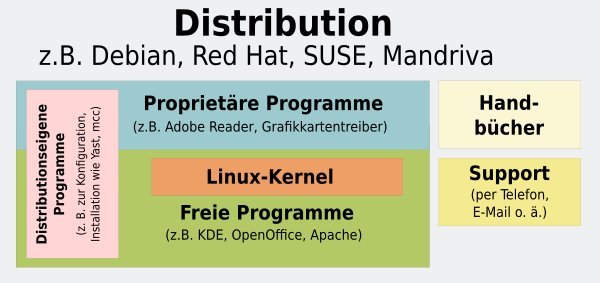
\includegraphics[scale=0.1]{images/distros1.jpg}}
	    \hspace{30px}
	    \fbox{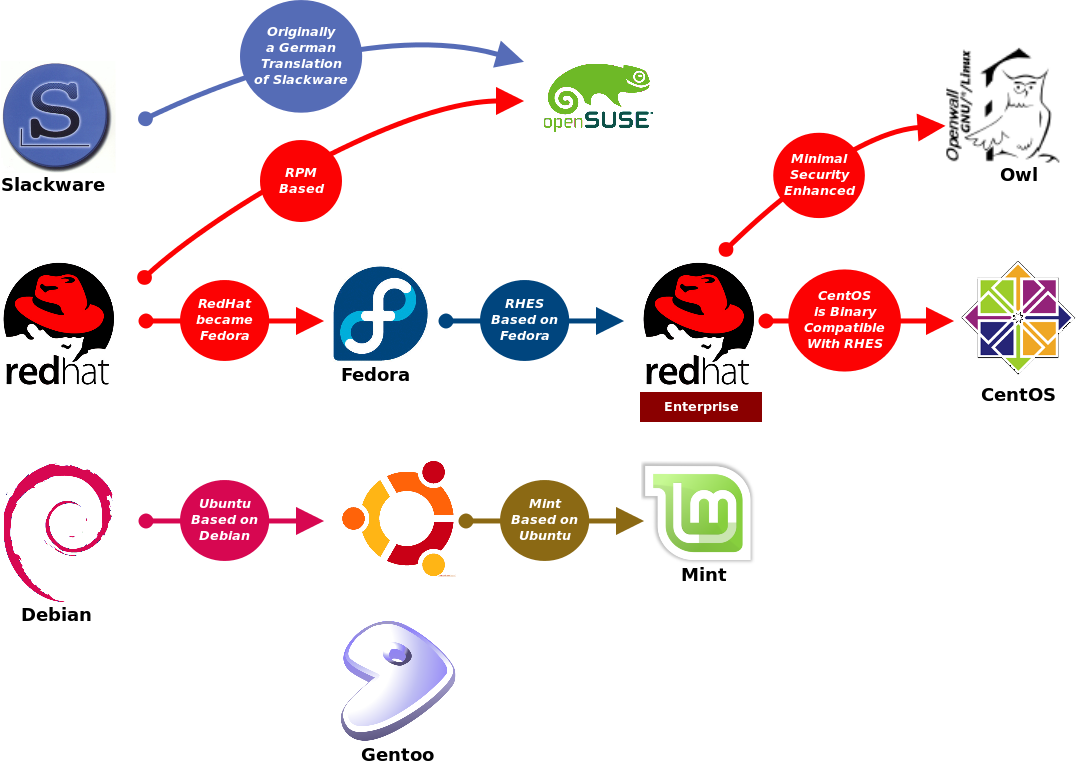
\includegraphics[scale=0.1]{images/distros2.png}}
	    \hspace{30px}
	\end{figure}
\end{frame}

\begin{frame}
	\frametitle{Organización física de discos}
	\begin{figure}
	    \fbox{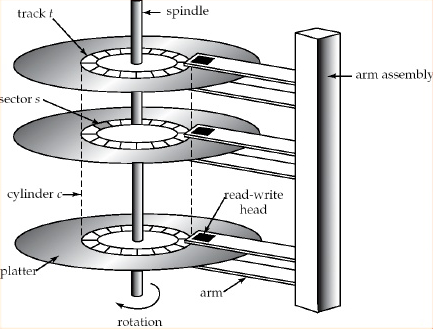
\includegraphics[scale=0.5]{images/hdd1.jpg}}
	\end{figure}
\end{frame}

\begin{frame}
	\frametitle{Organización física de discos (cont.)}
	\begin{figure}
	    \fbox{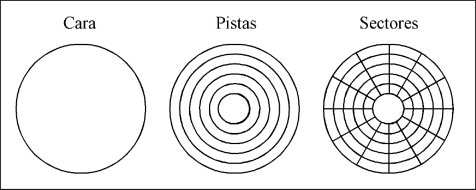
\includegraphics[scale=0.5]{images/hdd2.jpg}}
	\end{figure}
\end{frame}

\begin{frame}
	\frametitle{Organización física de discos (cont.)}
	\begin{figure}
	    \fbox{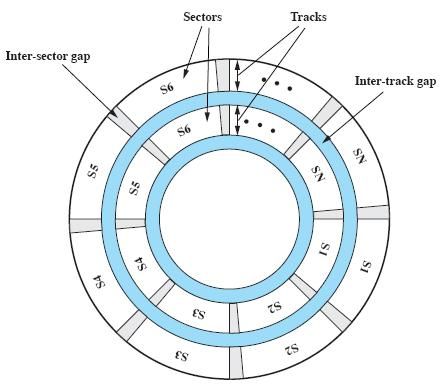
\includegraphics[scale=0.4]{images/hdd3.jpeg}}
	\end{figure}
\end{frame}